% Result figures. Curves and ROC/PR fit one column at their natural size;
% the four confusion panels need the full page width.

\begin{figure}[tb]
    \centering
    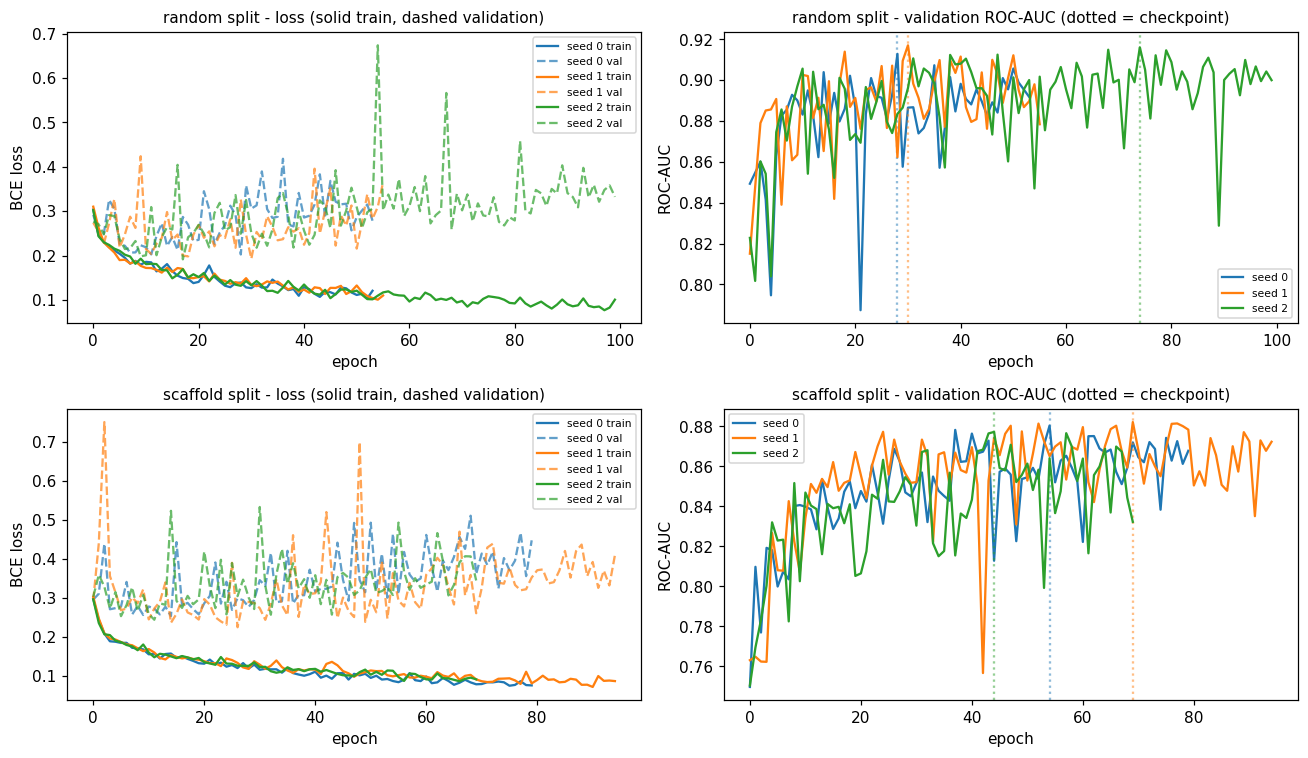
\includegraphics[width=0.92\columnwidth]{Images/training-curves.png}
    \caption{%
        All six runs. Left: training loss (solid) and validation loss (dashed). Right: validation ROC-AUC, the dotted line marking the restored checkpoint. Top row random split, bottom row scaffold; colour denotes the seed.
     }%
   \label{fig:curves}
\end{figure}

\begin{figure}[tb]
    \centering
    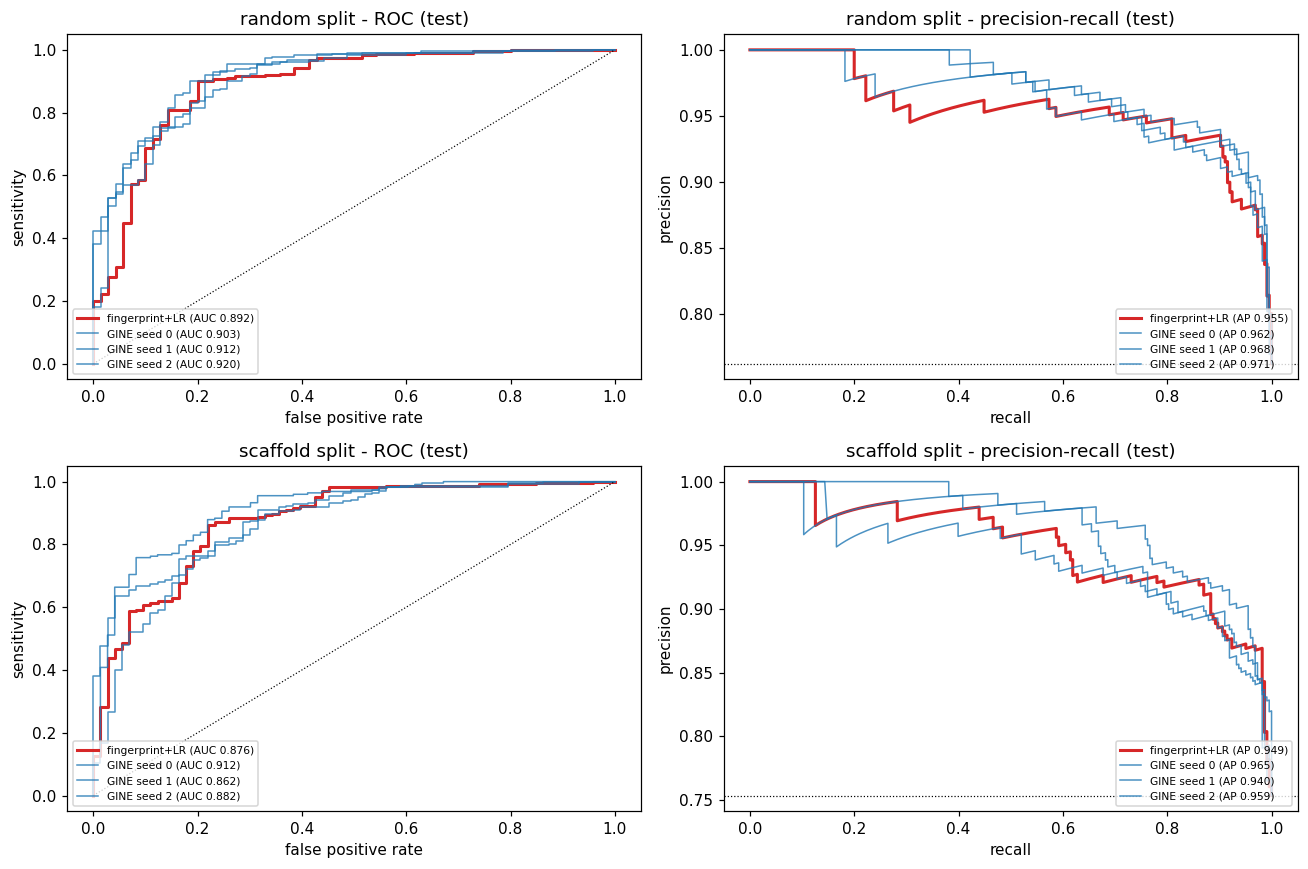
\includegraphics[width=0.90\columnwidth]{Images/roc-pr.png}
    \caption{%
        Test ROC (left) and precision--recall (right) curves. Red is the fingerprint baseline, blue the three network seeds; the dotted line marks the positive base rate.
     }%
   \label{fig:roc-pr}
\end{figure}

\begin{figure*}[tb]
    \centering
    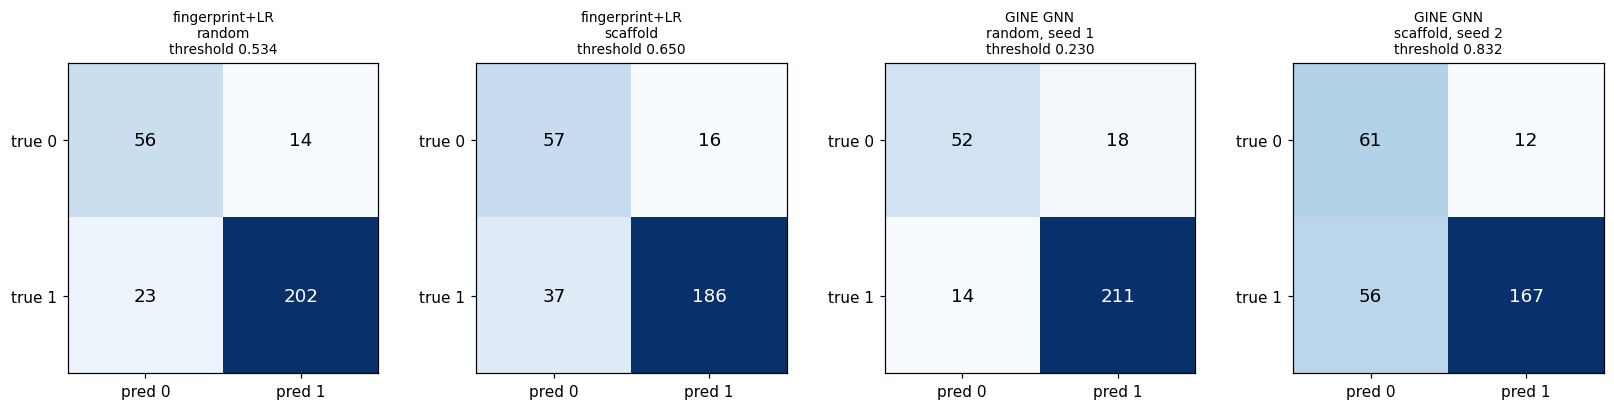
\includegraphics[width=0.60\textwidth]{Images/confusion.png}
    \caption{%
        Test confusion matrices at the frozen thresholds, using the seed with median test ROC-AUC for each split (seed 1 random, seed 2 scaffold).
     }%
   \label{fig:confusion}
\end{figure*}
